\chapter{Supplementary Diagnostics and Bidirectional Comparison}\label{app:diagnostics}

This appendix collects supplementary diagnostics for
Chapter~\ref{ch:experiments}: per-mechanism parameter figures,
per-architecture chunked-streaming results, and the LION versus
operator-level bidirectional comparison. Figure data are stored
alongside the corresponding scripts in the thesis figure folder.

\section{MSDC trained mixing weights}\label{app:diagnostics:msdc}

The MSDC diagnostic tracks trained mixing weights $\alpha_{d}$
for $d \in \{1, 2, 4, 8\}$. Divergence from the initial values
$\alpha_{1} = 1$ and $\alpha_{d > 1} = 0.01$ indicates that the
multi-dilation branches are exercised by the gradient.

\begin{figure}[!htbp]
\centering
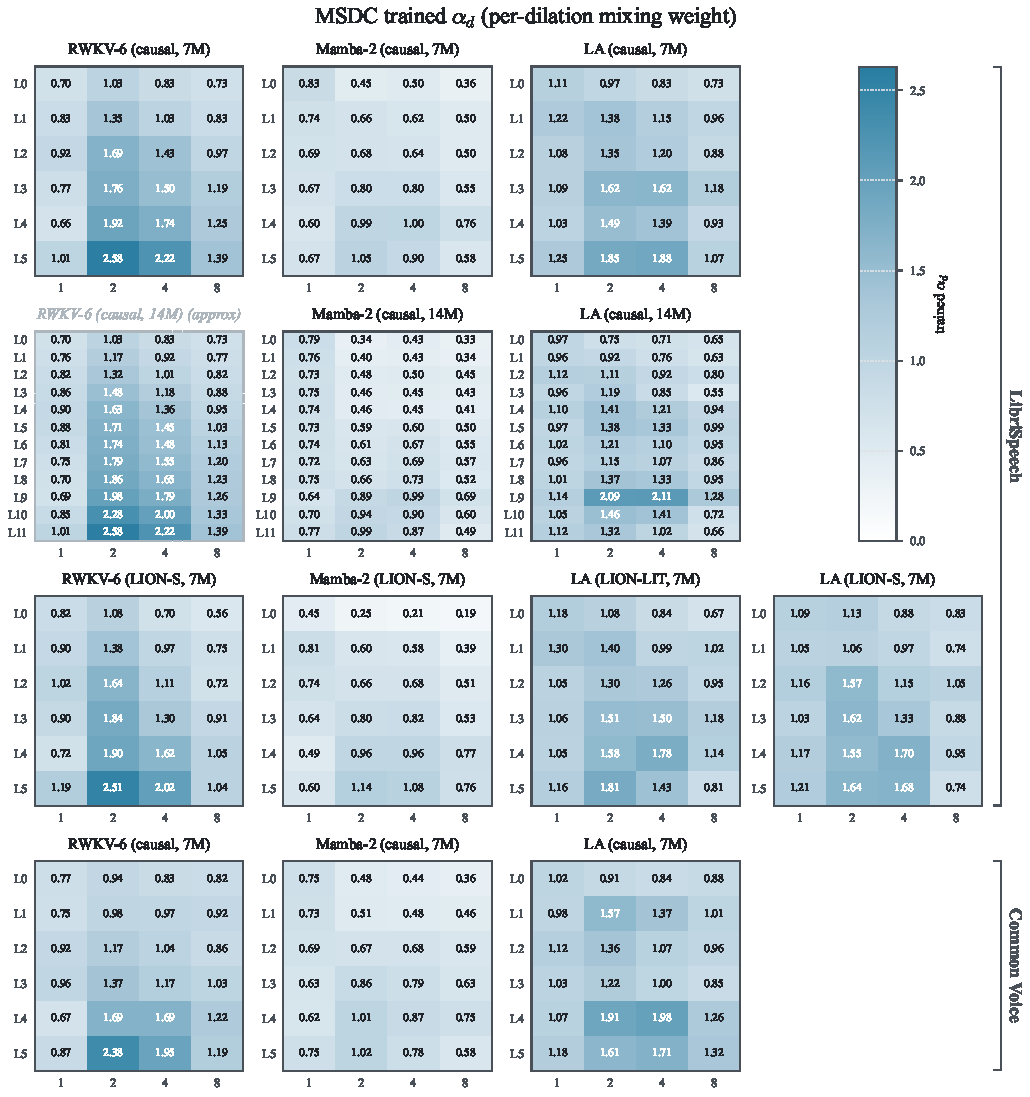
\includegraphics[width=0.9\linewidth]{figures/chapter5/F8_msdc_alpha_heatmaps.pdf}
\caption[MSDC trained $\alpha_{d}$ heatmaps]{Trained MSDC
$\alpha_{d}$ values at the 7M scale. Rows index encoder layers
and columns index dilations $\{1, 2, 4, 8\}$; non-initial
$\alpha_{d > 1}$ values indicate engaged multi-dilation
branches.}
\label{fig:app:msdc-alpha}
\end{figure}

\section{DHO rotation angle and viscosity diagnostics}\label{app:diagnostics:dho}

The DHO diagnostic tracks rotation angles $\theta_{t, h, b}$ and
viscosities $\eta_{h, b}$. Non-zero trained $\eta$ indicates
engaged Rayleigh dissipation; the realised $\theta$ distribution
is bounded by the depth-graded clip schedule of
Section~\ref{sec:proposed:dho}.

\begin{figure}[!htbp]
\centering
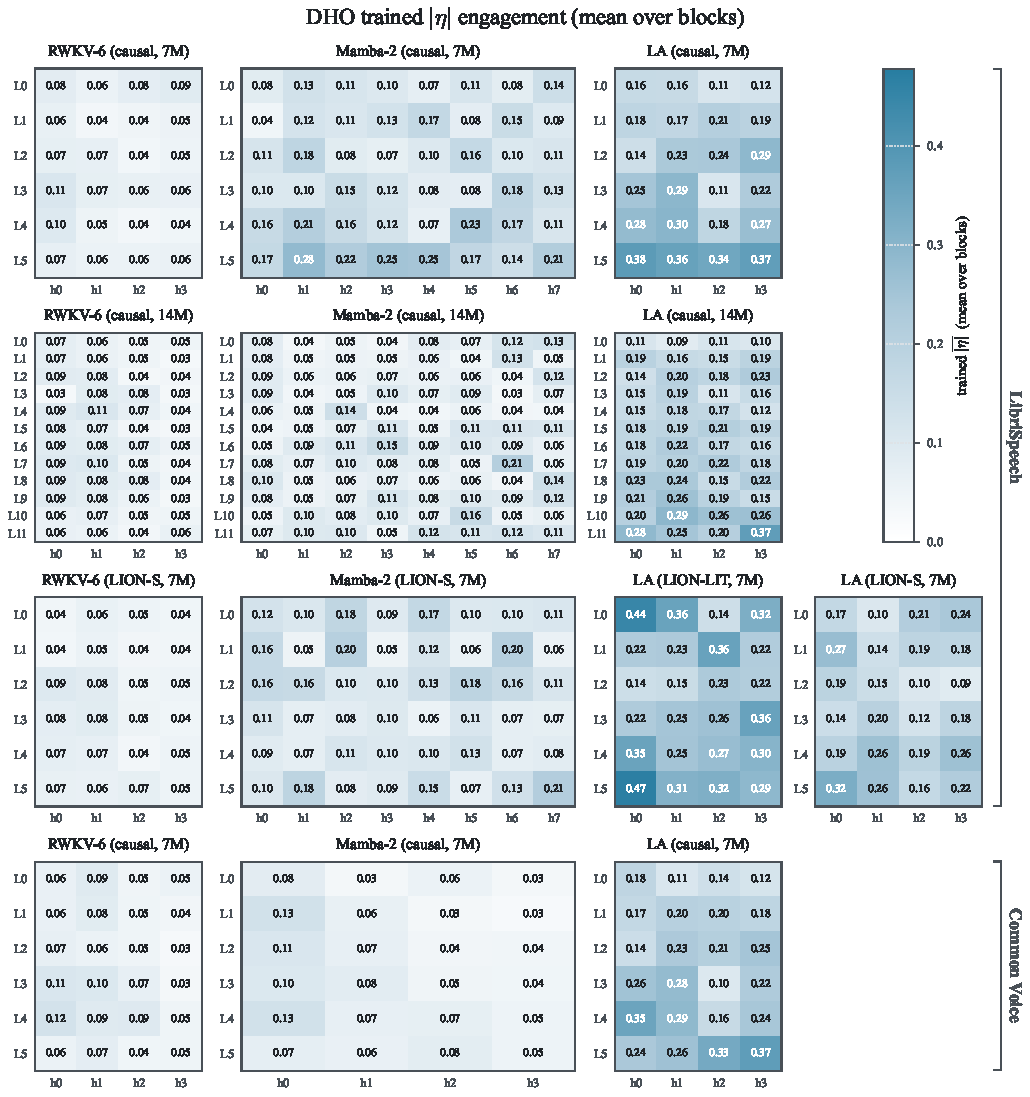
\includegraphics[width=0.9\linewidth]{figures/chapter5/F9_dho_eta_theta.pdf}
\caption[DHO $\eta$ and $\theta$ diagnostics]{DHO rotation-angle
and viscosity diagnostics across matrix cells. The realised
$\theta$ distribution reflects the depth-graded clip schedule;
trained $\eta$ indicates Rayleigh-coupling engagement.}
\label{fig:app:dho-eta-theta}
\end{figure}

\section{CVD per-head temperature heatmaps}\label{app:diagnostics:cvd}

The CVD diagnostic tracks the trained per-head temperature
$\tau_{h}$, which controls the strength of the chunk-local
key-similarity preconditioner.

\begin{figure}[!htbp]
\centering
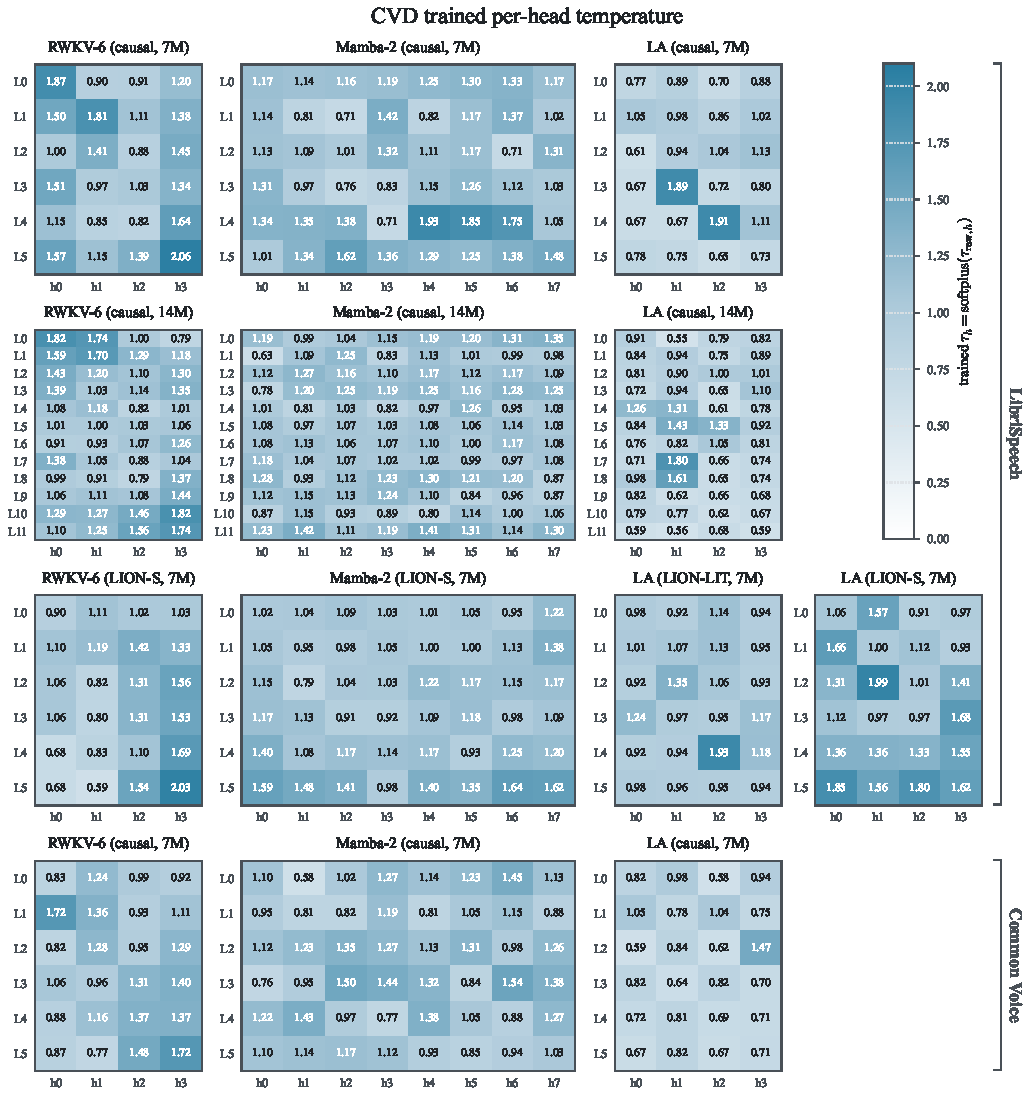
\includegraphics[width=0.9\linewidth]{figures/chapter5/F10_cvd_tau_heatmaps.pdf}
\caption[CVD per-head $\tau_{h}$ heatmaps]{Trained CVD
temperatures $\tau_{h}$ per layer and head across the
productive CVD deployments.}
\label{fig:app:cvd-tau}
\end{figure}

\section{Chunked-streaming evaluation per architecture}\label{app:diagnostics:chunked}

This figure gives the per-architecture breakdown of the
chunked-streaming evaluation summarised in
Table~\ref{tab:results:chunked-summary} of
Appendix~\ref{app:results}.

\begin{figure}[!htbp]
\centering
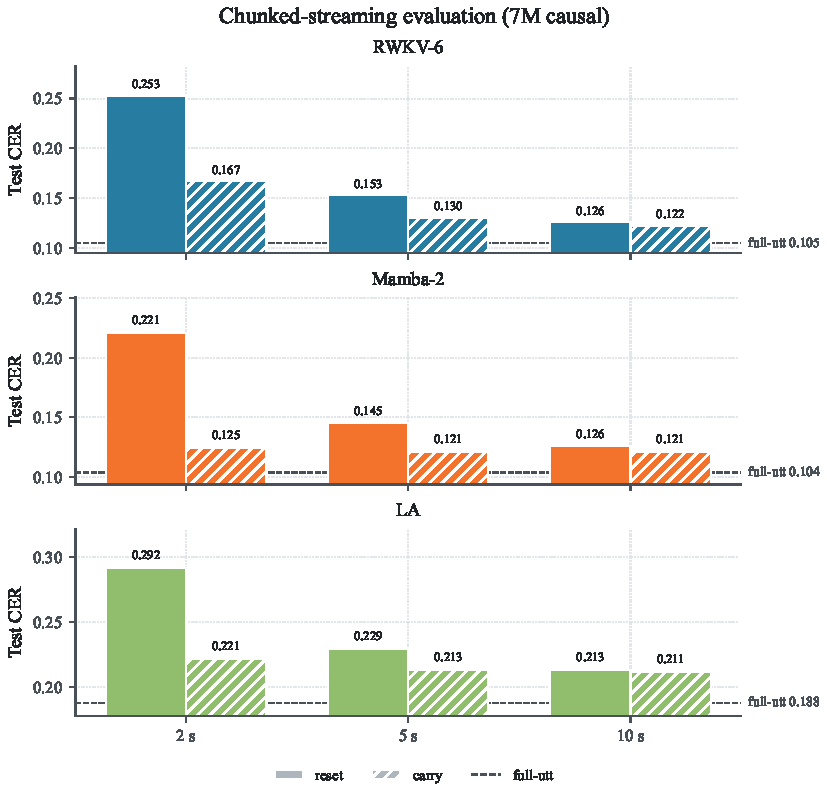
\includegraphics[width=0.9\linewidth]{figures/chapter5/F13_chunked_streaming.pdf}
\caption[Chunked-streaming per architecture]{Chunked-streaming
test CER for 7M causal cells under window sizes
$\{2.0, 5.0, 10.0\}$~s and reset/carry state policies, broken
out per architecture. Full-utterance CER is shown as the
reference.}
\label{fig:app:chunked}
\end{figure}

\section{Mechanism-level versus operator-level bidirectional adaptation}\label{app:diagnostics:lion-vs-vim}

The thesis uses LION~\citep{afzal2025linear} as the
mechanism-level bidirectional wrapper. This section compares it
with operator-level alternatives:
Bi-WKV~\cite{duan2024visionrwkv} runs the causal RWKV recurrence
forwards and backwards and combines the resulting hidden states;
Vision Mamba~\cite{zhu2024visionmamba} applies the same
forward-plus-backward template to selective state-space models.
Operator-level methods retain the linear-time envelope but pay
$2\times$ serial compute per layer; LION pays quadratic memory in
$T$ for the parallel attention but does not double the serial
compute. Every cell in
Table~\ref{tab:results:bidirectional-comparison-7m} is matched in
layer count and parameter count to its causal counterpart, with
the bidirectional mechanism replacing the causal scan in place.

\begin{table}[!htbp]
\centering
\small
\caption[LION versus operator-level bidirectional comparison, 7M]{
Matched 7M comparison between LION and operator-level
bidirectional adaptations. The LION column reports the natural
decay-class mapping and, for Linear Attention, the controlled
LION-S deployment. The $\Delta$ column is LION test CER minus
operator-level test CER within the same architecture row.}
\label{tab:results:bidirectional-comparison-7m}
\setlength{\tabcolsep}{6pt}
\renewcommand{\arraystretch}{1.15}
\begin{tabularx}{\linewidth}{@{}p{2.6cm} X r r r@{}}
\toprule
\textbf{Architecture} & \textbf{LION variant} &
\textbf{LION test} & \textbf{Operator-level test} &
\textbf{Δ (LION − op)} \\
\midrule
RWKV-6           & LION-S    & 0.0859 & 0.1062 (Bi-WKV) & $-0.0203$ \\
Mamba-2          & LION-S    & 0.0853 & 0.1221 (VIM)    & $-0.0368$ \\
Linear Attention & LION-LIT  & 0.2951 & 0.1858 (VIM)    & $+0.1093$ \\
Linear Attention & LION-S    & 0.1381 & 0.1858 (VIM)    & $-0.0477$ \\
\bottomrule
\end{tabularx}
\end{table}

\begin{table}[!htbp]
\centering
\small
\caption[Operator-level bidirectional reference at 14M]{
Operator-level bidirectional reference at the 14M scale. LION
14M cells are out of scope, so this table is operator-only.}
\label{tab:results:bidirectional-comparison-14m}
\setlength{\tabcolsep}{6pt}
\renewcommand{\arraystretch}{1.15}
\begin{tabularx}{\linewidth}{@{}X r r@{}}
\toprule
\textbf{Architecture (operator-level)} & \textbf{Test CER} & \textbf{Params} \\
\midrule
RWKV-6 with Bi-WKV       & 0.0738 & 13\,561\,117 \\
Mamba-2 with VIM         & 0.0746 & 12\,624\,445 \\
Linear Attention with VIM & 0.1207 & 10\,601\,245 \\
\bottomrule
\end{tabularx}
\end{table}

The reading at 7M is consistent across the family. On the two
backbones that carry native decay (RWKV-6 and Mamba-2), the
mechanism-level LION wrapper improves test CER by
$\Delta = -0.020$ to $-0.037$ over the operator-level alternative
at matched layers, parameters, and budget. On Linear Attention
the natural LION-LIT mapping has $\lambda = 1$ and no decay; it
loses to VIM by $\Delta = +0.109$. Adding decay through the
LION-S control reverses the result and yields $\Delta = -0.048$.
The pattern matches the decay-as-prerequisite finding of
Chapter~\ref{ch:experiments}; the LION wrapper's bidirectional
benefit on Linear Attention is conditional on a decay-bearing
mask, and the controlled LION-S deployment supplies that decay
through a per-token sigmoid that is not present in the underlying
causal backbone.

A complementary reading attaches to the 14M operator-level
reference of
Table~\ref{tab:results:bidirectional-comparison-14m}. The 14M
operator-level configuration runs twelve layers each carrying
its own forward+backward pairing, which is best read as twelve
bidirectional layer-equivalents at $2\times$ serial compute per
layer relative to a causal stack of the same parameter count.
The 7M LION-S rows are six layers; LION runs the bidirectional
access in parallel form within each layer, so the serial
compute per layer is the same as in the causal stack. On the
two backbones with native decay, the 14M operator-level
configuration reaches test CER values modestly below the
matched 7M LION-S rows: $0.0738$ on 14M RWKV-6 with Bi-WKV
against $0.0859$ on 7M RWKV-6 LION-S, and $0.0746$ on 14M
Mamba-2 with VIM against $0.0853$ on 7M Mamba-2 LION-S. The
mechanism-level LION wrapper at 7M therefore sits in
approximately the range the operator-level family reaches only
after doubling the parameter budget and doubling the
per-layer serial compute. The reading is that, on the two
backbones whose causal recurrence carries native decay, the
LION wrapper provides equivalent bidirectional expressivity at
roughly half the parameter and serial-compute budget; the
operator-level family's principal cost axis is the
doubled-per-layer serial computation rather than any
expressivity advantage at matched scale.

\section{Cross-scale persistence}\label{app:diagnostics:cross-scale}

Figure~\ref{fig:f5-cross-scale} supplements
Section~\ref{sec:experiments:lion} by visualising the causal-mode
test CER at 7M and 14M for each architecture-mechanism pair. The
underlying numbers are reported in
Table~\ref{tab:results:aggregated} and discussed per cell in the
main text.

\begin{figure}[!htbp]
\centering
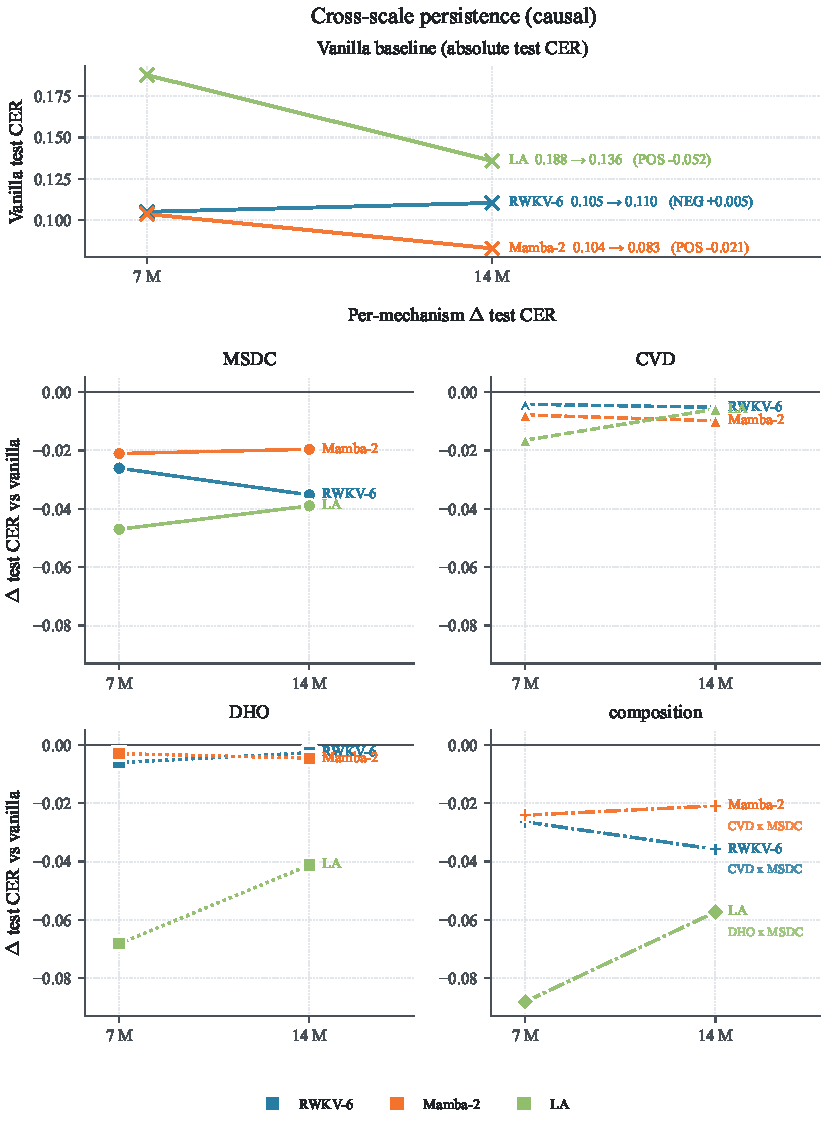
\includegraphics[width=0.9\linewidth]{figures/chapter5/F5_cross_scale_persistence.pdf}
\caption[Cross-scale persistence]{Causal-mode test CER at 7M and
14M for each architecture-mechanism pair. Lines connect the same
cell across scales.}
\label{fig:f5-cross-scale}
\end{figure}
